\chapter{Durchführung und Analyse}
Im fünften Kapitel erfolgt die Durchführung der Generierung von Tests mit \textit{Unitcraft} anhand verschiedener Projekte. Im Anschluss erfolgt eine Analyse der Ergebnisse, welche auf Basis zuvor definierter Metriken und eines klar definierten Bewertungsverfahren durchgeführt wird. Es findet eine Codeanalyse statt, welche auf Unterschiede in den Tests eingeht und anhand der Ergebnisse Schlüsse zieht. Abschließend werden die erzeugten Metriken mit den Metriken der menschlichen Tester verglichen.

\section{Durchführung}
Die Durchführung findet an einer Auswahl von Projekten mit unterschiedlichen Komplexitätsgraden und Größen statt. Die Projekte entstammen dem Unternehmen SENEC GmbH und werden mit ``Projekt x'' (x für eine Zahl) benannt. Projekt 1 besitzt eine Komplexität von 33 und ist mit einer Anzahl an Codezeilen von 318 das kleinste Projekt. Es folgt Projekt 2 mit einer Komplexität von 102 und einer Codezeilenanzahl von 730. Das größte und komplexeste Projekt ist Projekt 3. Die Komplexität beträgt 124 und die Zeilen an Quellcode 1231. [Tabelle \ref{fig:project}]\\\bgroup
\def\arraystretch{2}
\begin{table}[!h]
	\vspace{.5cm}
	\begin{center}
		\begin{tabular}{|c||c|c|c|}
			\hline 
			& Projekt 1 & Projekt 2 & Projekt 3 \\
			\hline 
			\hline
			Komplexität & 33 & 102 & 124 \\
			\hline
			Codezeilen & 318 & 730 & 1231 \\
			\hline
		\end{tabular} 
	\end{center}
	\caption{Testprojekte}
	\label{fig:project}
\end{table}
\egroupFür jedes Projekt werden 6 Testdurchläufe durchgeführt. Diese entstehen durch die Kombination von Prompt-Technik und dem Temperaturparameter. Somit wird der \textit{Zero-Shot} Prompt sowie der \textit{One-Shot} Prompt mit der Temperatur von 0, 0.25 und 0.5 für die Generierung verwendet. Insgesamt erzielen wir 18 Testdurchläufe, welche dafür sorgen, dass eine aussagekräftige Anzahl an Tests generiert wird.

\section{Evaluation der Tests}
Zur Bewertung und Analyse der Testergebnisse werden folgende Metriken benutzt: 
\begin{itemize}
    \setlength{\parskip}{1pt}
    \item Line Coverage
    \item Branch Coverage
    \item Overall Coverage
    \item Erfolgsquote mit Anzahl an Unit Tests
\end{itemize}
Jede Metrik wird projektweise evaluiert und bildet Durchschnittswerte aus allen Projekten. Anhand dieser Durchschnittswerte werden die Ergebnisse in Kategorien eingegliedert. Eine Einteilung der Coverage nach bestimmten Prozentwerten ist nicht sinnvoll, da es keinen Wert gibt, der auf alle Projekte zutrifft. Aufgrund dessen wird der Prozentbereich von 60\% - 90\% definiert und unterschieden, ob die Coverage in diesem angestrebten Bereich liegt (grün markiert) oder nicht (rot markiert). \cite{WhatReasonableCode}

\subsection{Line Coverage}
Tabelle \ref{fig:line-1} zeigt die Ergebnisse der Line Coverage für Projekt 1. Den besten Wert mit 72.4\% erzielt der \textit{Zero Shot} Prompt in Kombination mit einer Temperatur von 0.25. Der \textit{Zero-Shot} Prompt mit einer Temperatur von 0.5 schneidet mit 63.5\% am schlechtesten ab.
\bgroup
\def\arraystretch{2}
\begin{table}[H]
	\vspace{.5cm}
	\centering		
	\begin{center}
		\begin{tabular}{|c||c|c|c|}
			\hline 
			& 0 & 0.25 & 0.5 \\
			\hline 
			\hline
			\textit{Zero-Shot} & 71.4\% & \textbf{75.3\%} & 62.5\% \\
			\hline
			\textit{One-Shot} & 71.4\% & 66.2\% & 67.5\% \\
			\hline
		\end{tabular} 
	\end{center}
	\caption{\textit{Line Coverage} der generierten Tests für Projekt 1}
	\label{fig:line-1}
	\vspace{-.8cm}
\end{table}
\egroup
Die Ergebnisse der Line Coverage für Projekt 2 sind in Tabelle \ref{fig:line-2} dargestellt. Mit 84.9 \% erreicht der \textit{One-Shot} Prompt mit einer Temperatur von 0.25 den höchsten Wert. Der \textit{Zero-Shot} Prompt mit Temperatur 0 schneidet mit über 20\% schlechter ab.
\bgroup
\def\arraystretch{2}
\begin{table}[H]
	\vspace{.5cm}
	\centering		
	\begin{center}
		\begin{tabular}{|c||c|c|c|}
			\hline 
			& 0 & 0.25 & 0.5 \\
			\hline 
			\hline
			\textit{Zero-Shot} & 82.8\% & 61.3\% & 68.5\% \\
			\hline
			\textit{One-Shot} & 76.1\% & \textbf{84.9\%} & 83.2\% \\
			\hline
		\end{tabular} 
	\end{center}
	\caption{\textit{Line Coverage} der generierten Tests für Projekt 2}
	\label{fig:line-2}
	\vspace{-.8cm}
\end{table}
\egroup
Tabelle \ref{fig:line-3} stellt die Ergebnisse der Line Coverage für Projekt 3 dar. Mit 62.7\% erzielt der \textit{One-Shot} Prompt mit einer Temperatur von 0 den besten Wert. Der schlechteste Wert ist 47.3\% und entsteht in der Kombination aus \textit{One-Shot} Prompt und einer Temperatur von 0.5.
\bgroup
\def\arraystretch{2}
\begin{table}[H]
	\vspace{.5cm}
	\centering		
	\begin{center}
		\begin{tabular}{|c||c|c|c|}
			\hline 
			& 0 & 0.25 & 0.5 \\
			\hline 
			\hline
			\textit{Zero-Shot} & 42.7\% & 50.3\% & 55.3\% \\
			\hline
			\textit{One-Shot} & \textbf{62.7\%} & 60.7\% & 47.3\% \\
			\hline
		\end{tabular} 
	\end{center}
	\caption{\textit{Line Coverage} der generierten Tests für Projekt 3}
	\label{fig:line-3}
	\vspace{-.8cm}
\end{table}
\egroup
In Tabelle \ref{fig:line-avg} ist der Durchschnitt aller Ergebnisse dargestellt. Alle Werte treffen den angestrebten Bereich von 60\% - 90\%. Den besten Wert erreicht der \textit{One-Shot} Prompt mit einer Temperatur von 0.25. Am schlechtesten schneidet der \textit{Zero-Shot} Prompt mit einer Temperatur von 0.5 ab. Es ist klar erkennbar, dass eine hohe Temperatur wie 0.5, im Vergleich zum Rest deutlich schlechter abschneidet. Auch der \textit{One-Shot} Prompt erreicht im Vergleich zum \textit{Zero-Shot} Prompt die besseren Ergebnisse. 
\bgroup
\def\arraystretch{2}
\begin{table}[H]
	\vspace{.5cm}
	\centering		
	\begin{center}
		\begin{tabular}{|c||c|c|c|}
			\hline 
			& 0 & 0.25 & 0.5 \\
			\hline 
			\hline
			Zero-Shot & \colorbox{green}{65.6\%} & \colorbox{green}{62.3\%} & \colorbox{green}{62.1\%} \\
			\hline
			One-Shot & \colorbox{green}{70.1\%} & \colorbox{green}{\textbf{70.6\%}} & \colorbox{green}{66.0\%} \\
			\hline
		\end{tabular} 
	\end{center}
	\caption{Durchschnittliche Line Coverage der generierten Tests}
	\label{fig:line-avg}
	\vspace{-.8cm}
\end{table}
\egroup

\subsection{Branch Coverage}
Wie in Tabelle \ref{fig:branch-1} dargestellt, beträgt die Branch Coverage für Projekt 1 in allen Kombinationen 50.0\%. Somit schneidet jeder Prompt gleich ab.
\bgroup
\def\arraystretch{2}
\begin{table}[H]
	\vspace{.5cm}
	\centering		
	\begin{center}
		\begin{tabular}{|c||c|c|c|}
			\hline 
			& 0 & 0.25 & 0.5 \\
			\hline 
			\hline
			Zero-Shot & 50.0\% & 50.0\% & 50.0\% \\
			\hline
			One-Shot & 50.0\% & 50.0\% & 50.0\% \\
			\hline
		\end{tabular} 
	\end{center}
	\caption{Branch Coverage der generierten Tests für Projekt 1}
	\label{fig:branch-1}
	\vspace{-.8cm}
\end{table}
\egroup
In Tabelle \ref{fig:branch-2} erreicht der \textit{One-Shot} Prompt mit einer Temperatur von 0.25 erneut das beste Ergebnis der Branch Coverage für Projekt 2 und sticht im Vergleich zum Rest klar hervor.
\bgroup
\def\arraystretch{2}
\begin{table}[H]
	\vspace{.5cm}
	\centering		
	\begin{center}
		\begin{tabular}{|c||c|c|c|}
			\hline 
			& 0 & 0.25 & 0.5 \\
			\hline 
			\hline
			Zero-Shot & 67.0\% & 53.2\% & 57.4\% \\
			\hline
			One-Shot & 51.1\% & \textbf{71.3\%} & 59.6\% \\
			\hline
		\end{tabular} 
	\end{center}
	\caption{Branch Coverage der generierten Tests für Projekt 2}
	\label{fig:branch-2}
	\vspace{-.8cm}
\end{table}
\egroup
Für Projekt 3 fallen die Werte erheblich schlechter aus. Der \textit{One-Shot} Prompt erzielt mit 32.0\% und einer Temperatur von 0 das beste Ergebnis. Die Temperatur von 0.5 schneidet am schlechtesten ab.
\bgroup
\def\arraystretch{2}
\begin{table}[H]
	\vspace{.5cm}
	\centering		
	\begin{center}
		\begin{tabular}{|c||c|c|c|}
			\hline 
			& 0 & 0.25 & 0.5 \\
			\hline 
			\hline
			Zero-Shot & 24.2\% & 29.7\% & 22.7\% \\
			\hline
			One-Shot & \textbf{32.0\%} & 31.3\% & 22.7\% \\
			\hline
		\end{tabular} 
	\end{center}
	\caption{Branch Coverage der generierten Tests für Projekt 3}
	\label{fig:branch-3}
	\vspace{-.8cm}
\end{table}
\egroup
Tabelle \ref{fig:branch-avg} zeigt die Durchschnittswerte der Branch Coverage. Es ist eine klare Verschlechterung im Vergleich zur Line Coverage zu erkennen. Im Schnitt erreicht der \textit{One-Shot} Prompt mit der Temperatur 0.25 erneut den besten Wert. Auch der \textit{Zero-Shot} Prompt schneidet in Kombination mit einer Temperatur von 0.5 am schlechtesten ab. Des Weiteren wird deutlich, dass die Temperatur von 0.5 die schlechtesten Werte erzielt. Der Vergleich der Prompts ist ausgeglichener als zuvor, jedoch liegen alle Ergebnisse unter dem vorher festgelegten Idealbereich. 
\bgroup
\def\arraystretch{2}
\begin{table}[H]
	\vspace{.5cm}
	\centering		
	\begin{center}
		\begin{tabular}{|c||c|c|c|}
			\hline 
			& 0 & 0.25 & 0.5 \\
			\hline 
			\hline
			\textit{Zero-Shot} & \colorbox{red}{47.1\%} & \colorbox{red}{44.3\%} & \colorbox{red}{43.4\%} \\
			\hline
			\textit{One-Shot} & \colorbox{red}{44.4\%} & \colorbox{red}{\textbf{50.9\%}} & \colorbox{red}{44.1\%} \\
			\hline
		\end{tabular} 
	\end{center}
	\caption{Durchschnittliche \textit{Branch Coverage} der generierten Tests}
	\label{fig:branch-avg}
	\vspace{-.8cm}
\end{table}
\egroup

\subsection{Overall Coverage}
Tabelle \ref{fig:o-1} stellt die Overall Coverage Ergebnisse für Projekt 1 dar. 72.4\% ist der Höchstwert, erreicht durch die Kombination aus \textit{Zero-Shot} und der Temperatur 0.25. Die Temperatur 0.5 liefert wie schon bei der Line Coverage die schlechtesten Ergebnisse. Betrachtet man die Werte im Gesamten, erreicht das Sprachmodell ein zufriedenstellendes Ergebnis, da kein Wert unter 60\% fällt.
\bgroup
\def\arraystretch{2}
\begin{table}[H]
	\vspace{.5cm}
	\centering		
	\begin{center}
		\begin{tabular}{|c||c|c|c|}
			\hline 
			& 0 & 0.25 & 0.5 \\
			\hline 
			\hline
			\textit{Zero-Shot} & 69.0\% & \textbf{72.4\%} & 63.5\% \\
			\hline
			\textit{One-Shot} & 69.0\% & 64.4\% & 65.5\% \\
			\hline
		\end{tabular} 
	\end{center}
	\caption{\textit{Overall Coverage} der generierten Tests für Projekt 1}
	\label{fig:o-1}
	\vspace{-.8cm}
\end{table}
\egroup
Mit einer Overall Coverage von 81.0\% erzielt die Kombination aus \textit{One-Shot} Prompt und einer Temperatur von 0.25 den besten Wert für Projekt 2. [Tabelle \ref{fig:o-2}] Der schlechteste Wert beträgt 59.0\% und liegt somit unter der 60\% Grenze. Der Rest erreicht ein zufriedenstellendes Ergebnis.
\bgroup
\def\arraystretch{2}
\begin{table}[H]
	\vspace{.5cm}
	\centering		
	\begin{center}
		\begin{tabular}{|c||c|c|c|}
			\hline 
			& 0 & 0.25 & 0.5 \\
			\hline 
			\hline
			\textit{Zero-Shot} & 78.3\% & 59.0\% & 65.4\% \\
			\hline
			\textit{One-Shot} & 69.0\% & \textbf{81.0\%} & 76.5\% \\
			\hline
		\end{tabular} 
	\end{center}
	\caption{\textit{Overall Coverage} der generierten Tests für Projekt 2}
	\label{fig:o-2}
	\vspace{-.8cm}
\end{table}
\egroup
Eine klare Verschlechterung erkennt man im komplexesten und größten Projekt, dem Projekt 3. Tabelle \ref{fig:o-3} stellt die Ergebnisse tabellarisch dar. Es wird direkt erkennbar, dass keine Kombination die 60\% erreicht, und der höchste Wert bei einer Coverage von 53.5\% liegt. Hier wird deutlich, dass sich die Ergebnisse des Sprachmodells bei zunehmender Komplexität verschlechtern.
\bgroup
\def\arraystretch{2}
\begin{table}[H]
	\vspace{.5cm}
	\centering		
	\begin{center}
		\begin{tabular}{|c||c|c|c|}
			\hline 
			& 0 & 0.25 & 0.5 \\
			\hline 
			\hline
			Zero-Shot & 37.1\% & 44.2\% & 45.6\% \\
			\hline
			One-Shot & \textbf{53.5\%} & 51.9\% & 40.0\% \\
			\hline
		\end{tabular} 
	\end{center}
	\caption{Overall Coverage der generierten Tests für Projekt 3}
	\label{fig:o-3}
	\vspace{-.8cm}
\end{table}
\egroup
Tabelle \ref{fig:o-avg} zeigt die Durchschnittswerte und verdeutlicht ein zufriedenstellendes Ergebnis, da 3 von 6 Ergebnissen den angestrebten Bereich erreichen. Wie auch in den vorherigen Metriken, erzielt die Kombination aus \textit{One-Shot} Prompt und der Temperatur 0.25 den besten Wert. Die Temperatur von 0.5 erlangt die schlechtesten Ergebnisse und der \textit{One-Shot} Prompt ist dem \textit{Zero-Shot} Prompt sichtbar überlegen.
\bgroup
\def\arraystretch{2}
\begin{table}[H]
	\vspace{.5cm}
	\centering		
	\begin{center}
		\begin{tabular}{|c||c|c|c|}
			\hline 
			& 0 & 0.25 & 0.5 \\
			\hline 
			\hline
			Zero-Shot & \colorbox{green}{61.5\%} & \colorbox{red}{58.5\%} & \colorbox{red}{58.2\%} \\
			\hline
			One-Shot & \colorbox{green}{63.8\%} & \colorbox{green}{\textbf{65.8\%}} & \colorbox{green}{60.7\%} \\
			\hline
		\end{tabular} 
	\end{center}
	\caption{\textit{Average Overall Coverage} der generierten Tests}
	\label{fig:o-avg}
	\vspace{-.8cm}
\end{table}
\egroup

\subsection{Erfolgsquote}
Da die Erfolgsquote in allen Projekten ähnliche Werte aufweist und somit keine klare Unterscheidung aufgrund von Komplexität und Größe des Projektes getroffen werden kann, wird zur Evaluation dieser Quote der durchschnittliche Erfolg, auf Basis aller Projekte verwendet.\\
In Tabelle \ref{fig:succ} ist erkennbar, dass die Erfolgsquote zwischen 42.7\% (\textit{Zero-Shot} Prompt mit Temperatur von 0.5) und 46.0\% (\textit{One-Shot} Prompt mit Temperatur von 0.25) liegt. \bgroup
\def\arraystretch{2}
\begin{table}[H]
	\vspace{.5cm}
	\centering		
	\begin{center}
		\begin{tabular}{|c||c|c|c|}
			\hline 
			& 0 & 0.25 & 0.5 \\
			\hline 
			\hline
			Zero-Shot & 45.9\% & 45.9\% & 42.7\% \\
			\hline
			One-Shot & 43.0\% & \textbf{46.0\%} & 45.6\% \\
			\hline
		\end{tabular} 
	\end{center}
	\caption{Durchschnittliche Erfolgsquote der generierten Test}
	\label{fig:succ}
	\vspace{-.8cm}
\end{table}
\egroupDie in Tabelle \ref{fig:unit} dargestellten durchschnittlich erzeugten Unit Tests dienen der Berechnung der tatsächlich erfolgreichen Tests.\bgroup
\def\arraystretch{2}
\begin{table}[H]
	\vspace{.5cm}
	\centering		
	\begin{center}
		\begin{tabular}{|c||c|c|c|}
			\hline 
			& 0 & 0.25 & 0.5 \\
			\hline 
			\hline
			Zero-Shot & 52 & 59 & 57 \\
			\hline
			One-Shot & 45 & 45 & 44 \\
			\hline
		\end{tabular} 
	\end{center}
	\caption{Durchschnittliche Anzahl der generierten Test}
	\label{fig:unit}
	\vspace{-.8cm}
\end{table}
\egroupDabei multiplizieren wir die Anzahl der Unit Tests mit der Erfolgsquote. Das Ergebnis in Tabelle \ref{fig:succ-unit} stellt die tatsächlich erfolgreichen Unit Tests dar, die nicht aufgrund eines Erros während der Ausführung fehlschlugen. \bgroup
\def\arraystretch{2}
\begin{table}[H]
	\vspace{.5cm}
	\centering		
	\begin{center}
		\begin{tabular}{|c||c|c|c|}
			\hline 
			& 0 & 0.25 & 0.5 \\
			\hline 
			\hline
			\textit{Zero-Shot} & 23.9 & 27 & 24.3 \\
			\hline
			\textit{One-Shot} & 19.4 & 20.7 & 20.1 \\
			\hline
		\end{tabular} 
	\end{center}
	\caption{Durchschnittliche Anzahl erfolgreicher Tests}
	\label{fig:succ-unit}
	\vspace{-.8cm}
\end{table}
\egroup Es wird deutlich, dass weniger als die Häflte der generierten Unit Tests erfolgreich ausgeführt werden. Dadurch entsteht ein großer Anteil an irrelevantem Code im Projekt, was die Quellcode- sowie Projektqualität erheblich verschlechtert. Aus einem anderen Blickwinkel wird ebenso Potenzial für die Testabdeckung verschwendet, wenn ein Unit Test aufgrund eines simplen Errors wie bspw. einer \textit{NullPointerException} fehlerhaft ist.

\section{Testcodeanalyse}
Tabelle \ref{fig:succ} verdeutlicht, dass sich die Erfolgsquote aller Kombinationen aus Prompt-Technik und Temperatur kaum unterscheiden. Daraus lässt sich erschließen, dass die Unterschiede in den Coverage-Ergebnissen nicht aus dem Erfolg der generierten Tests ableitbar sind. Eine genauerer Blick auf den Testcode ist notwendig, um Tabelle \ref{fig:o-avg} zu analysieren. Dazu wird der generierte Testcode mit der schlechtesten Overall Coverage (\textit{Zero-Shot} Prompt mit Temperatur von 0.5) sowie der besten Overall Coverage (\textit{One-Shot} Prompt mit Temperatur von 0.25) verglichen, um Unterschiede nachvollziehen zu können. Es wird deutlich, dass fehlende \textit{Packages}, \textit{Imports} und \textit{Private-Access-Errors} die stärksten Hürden darstellen und einen Kompilierfehler erzwingen, sodass der generierte Test von \textit{Unitcraft} gelöscht wird. \\\\
Quellcode \ref{lst:missing-package} zeigt ein solches Vergessen des Packages, welches ein \textit{Missing package statement: 'com.senec.emsrelay'} verursacht und somit ein erfolgreiches Kompilieren des Tests verhindert.\\
\lstinputlisting[caption=Fehlendes Package in Testklasse,captionpos=b,label={lst:missing-package},language=Java]{Assets/Code/Missing-Package.java}
In Quellcode \ref{lst:missing-import} ist ein fehlender \textit{Import} dargestellt, welcher ebenso einen Kompilierfehler verursacht, da die Methode \textit{assertEquals} somit nicht bereitgestellt und das Löschen der gesamten Testklasse erzwungen wird.\\
\lstinputlisting[caption=Fehlender Import in Testklasse,captionpos=b,label={lst:missing-import},language=Java]{Assets/Code/Missing-Import.java}
Obwohl alle Prompts so designt sind, dass die Verwendung von \textit{Reflection} für den Zugriff auf private Methoden oder Attribute empfohlen wird, ist vermehrt sichtbar, dass bei der Wahl der Temperatur von 0.5 diese Anweisung ignoriert und somit durch einen \textit{Privat-Access-Error} die Ausführung des Tests verhindert wird.\\
In Abbildung \ref{fig:temp} wird der Einfluss der Temperatur in Form einer Verschlechterung bei einem Anstieg über 0.25 erkennbar. \begin{figure}[ht]
    \vspace{0.3cm}
    \centering
    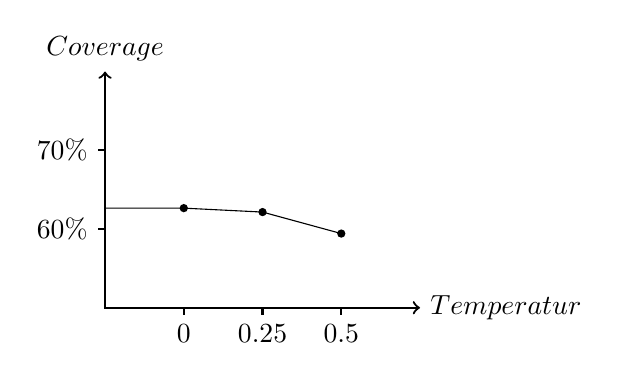
\begin{tikzpicture}
    \draw [<->,thick] (0,3) node (yaxis) [above] {$Coverage$}
        |- (4,0) node (xaxis) [right] {$Temperatur$};
    \draw (0,1.265) coordinate (a_1) -- (1,1.265) coordinate (a_2) -- (2,1.215) coordinate (a_3) -- (3, 0.942) coordinate (a_4);
    \draw[thick] (0, 1) -- (-0.09, 1) node[anchor=east] {60\%};
    \draw[thick] (0, 2) -- (-0.09, 2) node[anchor=east] {70\%};
    \draw[thick] (1, 0) -- (1, -0.09) node[anchor=north] {0};
    \draw[thick] (2, 0) -- (2, -0.09) node[anchor=north] {0.25};
    \draw[thick] (3, 0) -- (3, -0.09) node[anchor=north] {0.5};
    \coordinate (b) at (1,1.265);
    \fill[black] (a_2) circle (1.5pt);
    \fill[black] (a_3) circle (1.5pt);
    \fill[black] (a_4) circle (1.5pt);
    \end{tikzpicture}
    \caption{Einfluss der Temperatur auf die \textit{Coverage}}
    \label{fig:temp}
\end{figure}Betrachtet man die oben genannten Unterschiede im Testcode im Zusammenhang mit Abbildung \ref{fig:temp} kann man schlussfolgern, dass durch eine höhere Temperatur und somit einer höheren Kreativität der Fokus auf wichtige Aspekte verloren geht. Eine deterministischer Wert sorgt für bessere Ergebnisse in der Coverage. Die Auswertung der Daten in Tabelle \ref{fig:o-avg} zeigt jedoch, dass die Temperatur 0.25 in Kombination mit dem \textit{One-Shot} Prompt die beste Coverage erzielt. Dies verdeutlicht, dass durch einen geringen Anteil an Kreativität und mit zusätzlichem Beispielkontext durch die Prompt-Technik, unerwartete Hürden wie beispielsweise der Zugriff auf private Methoden oder zusätzlich notwendige Imports, besser gelöst werden können. Der Beispielkontext kann den Fokus auf wichtige Aspekte, trotz eines geringen Anteils an Kreativität, aufrechterhalten.\\\\
Somit nimmt nicht nur die Temperatur Einfluss auf die Lösung oben genannter Fehlerursachen. Abbildung \ref{fig:prompt} zeigt, dass der \textit{One-Shot} Prompt bessere Ergebnisse erzielt, als der \textit{Zero-Shot} Prompt \pgfplotstableread[row sep=\\,col sep=&]{
    Prompt & Value \\
    Zero Shot & 59.39 \\
    One Shot & 63.42 \\
    }\mydata

\begin{figure}[ht]
    \vspace{0.3cm}
    \centering
    \begin{tikzpicture}
        \begin{axis}[
            ybar,
            width=6cm,  % Adjust the width
            height=6cm,  % Adjust the height
            symbolic x coords={Zero Shot, One Shot},
            xtick=data,
            ymin=50,  % Set y axis minimum value
            ymax=70,  % Set y axis maximum value
            bar width=20pt,  % Adjust bar width
            nodes near coords,  % Display values on top of bars
            ylabel={Coverage (\%)},
            enlarge x limits=0.5,  % Reduce the space around the bars
        ]
        \addplot table[x=Prompt,y=Value]{\mydata};
        \end{axis}
    \end{tikzpicture}
    \caption{Einfluss des Prompts auf die Coverage}
    \label{fig:prompt}
\end{figure}Daraus lässt sich ableiten, dass durch das Hinzufügen eines Beispielkontextes innerhalb eines \textit{One-Shot} Prompts die oben genannten Hürden besser gelöst werden. Dies ist auf den zusätzlichen Kontext zurückführen, da dieser durch beispielhaft korrektes Einbinden von Imports und Packages eine Vorlage bietet.\\\\
Schlussfolgernd lässt sich sagen, dass beide Faktoren das Ergebnis maßgeblich beeinflussen sowie für die am Anfang genannten Testunterschiede sorgen. Der \textit{One-Shot} Prompt ist aufgrund seines zusätzlichen Kontextes dem \textit{Zero-Shot} Prompt überlegen. Vor allem in Kombination mit einer deterministischen Temperatur mit einem Anteil von Kreativität, welcher 0.25 nicht überschreitet, wurden die besten Ergebnisse erzielt. Die richtige Wahl von Prompt-Technik sowie Temperatur ist essenziell für die Lösung oben genannter Probleme.

\section{Vergleich mit manuellen Testergebnissen}
Im Folgenden werden die Testergebnisse zwischen den von \textit{Unitcraft} generierten Tests und denen, die in der Softwareentwicklung der SENEC GmbH manuell erstellt wurden, verglichen. Dabei wird das jeweilige beste Ergebnis des Sprachmodells genutzt, um das mögliche Potenzial im Vergleich zu den vom Menschen geschriebenen Tests aufzuzeigen.\\\\
Tabelle \ref{fig:comp} zeigt den direkten Vergleich der Metriken tabellarisch.\bgroup
\def\arraystretch{2}
\begin{table}[ht]
	\vspace{.5cm}
	\centering		
	\begin{center}
		\begin{tabular}{|c||c|c|c|}
			\hline 
			Projekt & Metrik & Manuell & GPT-4o \\
			\hline 
			\hline
			\textbf{1} & Line Coverage & \textbf{84.4\%} & 75.3\% \\
			\hline
			& Branch Coverage & 40.0\% & \textbf{50.0\%} \\
			\hline
			& Overall Coverage & \textbf{79.3\%} & 72.4\% \\
			\hline
			& Erfolgsquote & \textbf{100.0\%} & 50.0\% \\
			\hline
			\hline
			\textbf{2} & Line Coverage & 35.3\% & \textbf{84.9\%} \\
			\hline
			& Branch Coverage & 41.5\% & \textbf{71.3\%} \\
			\hline
			& Overall Coverage & 37.0\% & \textbf{81.0\%} \\
			\hline
			& Erfolgsquote & \textbf{100.0\%} & 72.6\%\\
			\hline
			\hline
			\textbf{3} & Line Coverage & 48.7\% & \textbf{62.7\%} \\
			\hline
			& Branch Coverage & 19.5\% & \textbf{32.0\%} \\
			\hline
			& Overall Coverage & 40.0\% & \textbf{53.5\%} \\
			\hline
			& Erfolgsquote & \textbf{100.0\%} & 43.9\% \\
			\hline
		\end{tabular} 
	\end{center}
	\caption{Vergleich der Metriken manueller Tests und generierter Tests}
	\label{fig:comp}
\end{table}
\egroupIm Projekt 1 erreichen die manuell geschriebenen Tests mit 84.4\% die bessere Line Coverage. Betrachtet man jedoch Projekt 2 und 3, wird deutlich, dass GPT-4o klar bessere Ergebnisse liefert. Speziell im 2. Projekt erreicht das Sprachmodell eine mehr als doppelt so gute Leistung. Beim Vergleich der Branch Coverage schneiden die Testergebnisse der manuellen Tester in allen Projekten schlechter ab. Auch hier sticht GPT-4o in Projekt 2 mit einer besonderen Leistung hervor. Ähnlich wie bei der Line Coverage erreichen die manuellen Tests in Projekt 1 knapp 7\% mehr Overall Coverage. Vergleicht man hierbei wieder mit Projekt 2 und 3 wird stark deutlich, dass GPT-4o besser performed. Wie schon in Tabelle \ref{fig:succ} analysiert, schneidet die Erfolgsquote des Sprachmodells schlecht ab. Insbesondere im direkten Vergleich entsteht eine große Differenz zwischen beiden Werten. Die manuellen Tests weisen eine Erfolgsquote von 100\% in jedem Projekt auf. Dies ist ein zu erwartender Wert, da beim manuellen Testen nur Tests im Projekt bleiben, die erfolgreich ausgeführt werden. Somit wird irrelevanter Testcode vermieden und die Qualität im Projekt gesichert.\\\\
Bei einer Gesamtbetrachtung aller Vergleiche zeigt sich, dass GPT-4o in 7 von 12 Metriken bessere Werte aufweist. Dies veranschaulicht das Potenzial des Sprachmodells beim Generieren von JUnit-Tests. Es wird jedoch auch deutlich, dass der Testcode von manuellen Tests eindeutig erfolgreicher in der Auführung und somit qualitativer ist, da im Schnitt weniger irrelevanter Testcode entsteht.
